%%
%% Automatically generated file from DocOnce source
%% (https://github.com/hplgit/doconce/)
%%
%%


%-------------------- begin preamble ----------------------

\documentclass[%
oneside,                 % oneside: electronic viewing, twoside: printing
final,                   % draft: marks overfull hboxes, figures with paths
10pt]{article}

\listfiles               %  print all files needed to compile this document


\usepackage[totoc]{idxlayout}   % for index in the toc
\usepackage[nottoc]{tocbibind}  % for references/bibliography in the toc

\usepackage{relsize,makeidx,color,setspace,amsmath,amsfonts,amssymb}
\usepackage[table]{xcolor}
\usepackage{bm,ltablex,microtype}
\usepackage{comment} 
\usepackage[pdftex]{graphicx}

\usepackage{fancyvrb} % packages needed for verbatim environments

\usepackage[T1]{fontenc}
%\usepackage[latin1]{inputenc}
\usepackage{ucs}
\usepackage[utf8x]{inputenc}

\usepackage{lmodern}         % Latin Modern fonts derived from Computer Modern


\usepackage{pgfplotstable, booktabs}

\pgfplotstableset{
    every head row/.style={before row=\toprule,after row=\midrule},
    every last row/.style={after row=\bottomrule}
}





% Hyperlinks in PDF:
\definecolor{linkcolor}{rgb}{0,0,0.4}
\usepackage{hyperref}
\hypersetup{
    breaklinks=true,
    colorlinks=true,
    linkcolor=linkcolor,
    urlcolor=linkcolor,
    citecolor=black,
    filecolor=black,
    %filecolor=blue,
    pdfmenubar=true,
    pdftoolbar=true,
    bookmarksdepth=3   % Uncomment (and tweak) for PDF bookmarks with more levels than the TOC
    }
%\hyperbaseurl{}   % hyperlinks are relative to this root

\setcounter{tocdepth}{2}  % levels in table of contents

% --- fancyhdr package for fancy headers ---
\usepackage{fancyhdr}
\fancyhf{} % sets both header and footer to nothing
\renewcommand{\headrulewidth}{0pt}
\fancyfoot[LE,RO]{\thepage}
% Ensure copyright on titlepage (article style) and chapter pages (book style)
\fancypagestyle{plain}{
  \fancyhf{}
  \fancyfoot[C]{{\footnotesize \copyright\ 1999-2018, "Computational Physics I FYS3150/FYS4150":"http://www.uio.no/studier/emner/matnat/fys/FYS3150/index-eng.html". Released under CC Attribution-NonCommercial 4.0 license}}
%  \renewcommand{\footrulewidth}{0mm}
  \renewcommand{\headrulewidth}{0mm}
}
% Ensure copyright on titlepages with \thispagestyle{empty}
\fancypagestyle{empty}{
  \fancyhf{}
  \fancyfoot[C]{{ }}
  \renewcommand{\footrulewidth}{0mm}
  \renewcommand{\headrulewidth}{0mm}
}

\pagestyle{fancy}


% prevent orhpans and widows
\clubpenalty = 10000
\widowpenalty = 10000

% --- end of standard preamble for documents ---


% insert custom LaTeX commands...

\raggedbottom
\makeindex
\usepackage[totoc]{idxlayout}   % for index in the toc
\usepackage[nottoc]{tocbibind}  % for references/bibliography in the toc
\usepackage{listings}
\usepackage[normalem]{ulem} 	%for tables
\useunder{\uline}{\ul}{}
\usepackage{hyperref}
\usepackage[section]{placeins} %force figs in section

\usepackage{natbib}


%-------------------- end preamble ----------------------

\begin{document}

% matching end for #ifdef PREAMBLE

\newcommand{\exercisesection}[1]{\subsection*{#1}}


% ------------------- main content ----------------------



% ----------------- title -------------------------

\thispagestyle{empty}

\begin{center}
{\LARGE\bf
\begin{spacing}{1.25}
Numerically solving linear diffusion problems with Dirichlet boundary conditions
\end{spacing}
}
\end{center}

% ----------------- author(s) -------------------------

\begin{center}
{\bf Johan Nereng}
\end{center}

    \begin{center}
% List of all institutions:
\centerline{{\small Department of Physics, University of Oslo, Norway}}
\end{center}
    
% ----------------- end author(s) -------------------------

% --- begin date ---
\begin{center}
Nov 21, 2018
\end{center}
% --- end date ---

\vspace{1cm}
\begin{abstract}
AOooo
\end{abstract}



\section{Introduction}
When a system is in a state where the spatial density distribution of some quantity is unequilibrated, a flow from regions of high density to regions of low density occurs. This phenomenon, known as diffusion, is described by Fick's first law, named after the German physician Adolf Eugen Fick. Fick's first law states that the diffusional flux \footnote{The diffusional flux is the quantity transport per unit time per unit area, perpendicular to the direction of the diffusion} is proportional to the concentration gradient of the diffusing component \citep[pp. 339-340]{MatSci}. Less precisely, it can be said that the strength of the diffusional flow at a specific place, corresponds to how strongly the density varies around that place. Application of a conservation law appropriate to the diffusing quantity leads to what is either known as Fick's second law, or the continuity equation \citep[pp.341-342]{MatSci}). \\
The continuity equation, may, under the constraints of linearity between gradient and flow, be expressed as the partial differential equation (PDE) known as the heat equation. Diffusion problems where one can assume such linearity may be expressed through \eqref{eq:HeateqGEN}. Typically, such linearity is the domain of bodies with uniform properties. Along with the appropriate initial conditions (ICs) and boundary conditions (BCs), the closed form solution of the PDE may sometimes be obtained using certain methods, of which some are outlined later in this project. However, when describing real physical systems, such closed form solution are often not obtainable, yet the same computational procedures may often be applied in providing a numerical solution. Finite-difference methods (FDM) are perhaps the most commonly applied type of method for solving PDEs. In short, FDMs are discretization methods in which the derivatives of a differential equation is approximated using by finite differences \citep[p. 46]{compPDE}, usually obtained through a Taylor expansion. \newline

The starting point for project, heat equation problem, to which a closed form solution (CFS) is obtainable. Subsequently, the three FDMs are itnroduced and explained, algorithms developed, and tested on the PDE and compared to CFS.   especially chosen because it has relatively easily obtainable closed form solution. 



WHY scale the problem
Application of this heat equation to a simple system of heat flow in a rod is the basis for this project, which aims examine finite sums numerical methods for linear diffusion problems with Dirichlet boundary conditions (BCs) - or more simply put, fixed boundary conditions. \newline

What is finite difference method? How to make a such a solver that can be applied to a range of problems? - scaling!

 
1: look at the heat equation. What's what, when does it apply? \newline

2: How to scale a heat equation problem? \newline
 
3. What is the problem we are looking at? A general case. Many problems may be expressed as this through the scaling methods described above.  \newline
 
4. Analytical solution -> With these system properties, it is fairly easily calculated. Other times, not necessarily so. That's why numerical solutions are desirable.  \newline

5. Discretize problem from 3. \newline
 

For the purpose of approximating the derivatives of $u$, three methods are applied: explicit forward Euler, implicit Backward Euler, and the implicit Crank-Nicolson with a time-centered scheme.



The diffusion equation, which provides a connection between a diffusion rate and a concen time derivative temperature relation to curvature

dy with non-uniform temperature, the thermal energy - or he


Initial conditions, boundry conditions \newline
The dimensionsless Heat Equation -> the heat equation
1+1 d-> 1d
assumes regular stuff about math


\section{Methods}
\subsection{The Heat Equation}
\label{M.1DHQ}
The heat equation \eqref{eq:HeateqGEN}, also known as the diffusion equation, is a special case of the continuity equation in which the relationship between flow and density gradient is linear \citep{HJ15}. A wide range of diffusion problems may, with sufficient simplifications, be expressed through this equation, and solved provided suitable ICs and BCs. These ICs represent the state of the system, or the distribution of the diffusive quantity , at $t=0$, while the BCs apply restrictions on the diffusion on the periphery of body in which the diffusion takes place.\newline
\begin{equation}
\frac{\partial u}{\partial t}=D \nabla^2 u
\label{eq:HeateqGEN}
\end{equation}
\textit{Where $u$ signifies the density of the diffusive quantity, $t$ the time, while $D=constant$ is a proportionality constant -  also known as the diffusion constant. } \newline

As an example of the application of the heat equation, consider a one dimensional system consisting of a rod of length $L$, with each end of the rod in contact with a thermal bath.  If $x$ denotes the spatial coordinates along the length of the rod, the thermal gradient, $u=u(x,t)$, is subject to heat diffusion unless equilibrated. Assume that the two thermal baths each hold one end of the rod at constant temperature; $u_0$ (at $x=0$) and $u_1=u_0 +\Delta u, \quad \Delta u>0$ (at $x=L$), where $\Delta u$ is the difference in temperature between the two heat baths. This means that the BCs are:
\begin{align}
u(0,t)=u_0, \quad t \geq 0 \\
u(L,t)=u_1, \quad t \geq 0
\end{align}
Furthermore, assume that the rod has thermally equilibrated with the heat bath holding temperature $u_0$ before $x=L$ is put into contact with the other thermal bath at $t=0$. Thus the ICs are:
\begin{equation}
u(x,0)=f(x)=  \begin{cases}
 & u_0, \quad 0\leq x < L\\
 & u_1, \quad x=l
  \end{cases}
\end{equation}

Lastly, the rod has the following uniform properties; thermal conductivity, $\kappa(W/(m\cdot K)$, specific heat capacity $c(J/(kg \cdot K))$, and (mass) density $\rho(kg/m^3)$, the diffusion constant $D$ may be expressed as $D=\frac{\kappa}{c \rho}$ \citep[p.304]{HJ15}. Assuming linear diffusion, the time evolution of heat distribution in the rod may then be expressed in terms of the heat equation \eqref{M.1DHQ}, which results in the following mathematical problem:

\begin{align}
PDE:&\quad \frac{\kappa}{c \rho}\frac{\partial^2 u(x,t)}{\partial x^2}=\frac{\partial u(x,t)}{\partial t} \label{eq:rod}\\
ICs:&\quad u(x,0)=f(x)=  \begin{cases}
  u_0, \quad 0\leq x < L\\
 u_1, \quad x=L
  \end{cases} \label{eq:rodIC}\\\
BCs:& \quad u(0,t)=u_0, \quad t \geq 0 \quad u(L,t)=T_1, \quad t \geq 0 \label{eq:rodBC}
\end{align}


\subsection{Scaling the Heat Equation}
Both the algorithms developed later in this project and the outlined method for obtaining a CFS, assumes a scaled diffusive problem. Scaling often requires considerable insight in the problem, on account of choosing suitable characteristic variables. The following outlined scaling procedures are from an MIT course on PDEs, and does not go into detail on choice of characteristic variables - the choice of which is left open (for more details see \cite{Hancock}). Below, heat is referred to the diffusive quantity, $u$. The procedure does however apply to other diffusive quantities involved in diffusion problems applicable to the heat/diffusion equation. \newline

First, dimensionless variables are introduced:
\begin{align}
\hat{x}=\frac{x}{L_*}, \qquad \hat{t}=\frac{t}{T_*}, \qquad \hat{u}(\hat{x},\hat{t})=\frac{u(x,t)}{U_*},  \qquad\hat{f}(\hat{x}) =\frac{f(x)}{U_x}
\end{align}
Where $[L_*]=L$, $[T_*]=T$, $[U_*]=U$ are characteristic length, time and temperature. Using the chain rule yields:
\begin{align*}
u_t=\frac{\partial u}{\partial t}=U_* \frac{\partial \hat{u}}{\partial \hat{t}}\frac{\partial \hat{t}}{\partial t}=\frac{U_*}{T_*}\frac{\partial \hat{u}}{\partial \hat{t}} 
\end{align*}
And similarly:
\begin{align*}
u_x=\frac{U_*}{L_*}\frac{\partial \hat{u}}{\hat{x}} \\
u_{xx}=\frac{U_*}{L_*^2}\frac{\partial^2 \hat{u}}{\hat{x}^2} \\
\end{align*}
Substitution into the heat equation \eqref{eq:HeateqGEN}:
\begin{align*}
u_t=D u_{xx} \quad \rightarrow \quad \frac{\partial \hat{u}}{\partial \hat{t}}= D \frac{T_*}{L_*}\frac{\partial^2 \hat{ u}}{\partial \hat{x}^2}
\end{align*}
Then, setting $T_*=L_*^2/D$ results in: 
\begin{align}
\frac{\partial \hat{u}}{\partial \hat t}=\frac{\partial^2 \hat{u}}{\partial \hat{x}^2} \label{eq:1dscaled}
\end{align}
\eqref{eq:1dscaled} now holds the scaled heat equation problem. All that is left is to similarly scale the ICs and BCs pertaining to the particular problem at hand.\newline

The scaling procedures above is now applied to the case of the one dimensional rod problem from the section \hyperref[M.1DHQ]{on the heat equation} - in the future simply referred to as the rod problem. The characteristic length of the problem is taken to be the length of the rod, so $L_*=L$. With the restrictions posed on the rod, $u_0$ ($u_0<u_1$) is the lowest temperature that any part of the rod may have, therefore $u_0$ is defined as $u=0$. This makes the the difference in temperature of the two thermal bath a natural choice for characteristic temperature, that is; $U_*=\Delta u$. Lastly, characteristic time is set to $T_*=L_*^2/D=L^2 \frac{\kappa}{c \rho}$. Renaming $\hat{u}$ as $u$, $\hat{t}$ as $t$ , and so on, then yields the following scaled diffusion problem:

\begin{align}
PDE:&\quad \frac{\partial^2 u(x,t)}{\partial x^2}=\frac{\partial u(x,t)}{\partial t} \label{eq:scaled.rod}\\
ICs:&\quad u(x,0)=f(x)=  \begin{cases}
  0, \quad 0 < x < 1\\
 1, \quad x=1
  \end{cases} \label{eq:scaled.rodIC}\\\
BCs:& \quad u(0,t)=0, \quad t \geq 0 \quad u(1,t)=1, \quad t \geq 0 \label{eq:scaled.rodBC}
\end{align}

\subsection{Approximation methods}
\label{M.ApproxMethods}
\textbf{ 
explicit: uses first order temporal, second order spatial. Solve directly for next step
implicit: uses first order temporal, second order spatial. Solve for previous step, use gaussian elimination, and solve matrix product for $Av=v_{j-1}$ for $v$.}

The approximation methods used in this project are the explicit forward Euler, the implicit Backward Euler, and the Crank-Nicolson scheme with a time-centered scheme. All of these three methods are FDMs, which means that they approximate derivatives  by using a sum of differences, where the terms in this case are obtained from Taylor series expansions of the function to be differentiated. The description of the methods in this project is restricted to the expressions involved in the scaled heat equation \eqref{eq:Approxim.heateq}, however application to other types of PDEs are readily available in literature such as the book by A. Tveito and R.Winther on PDEs in numerical computations \cite{compPDE}.
\begin{align}
PDE:& \quad \frac{\partial^2 u(x,t)}{\partial x^2}=\frac{\partial u(x,t)}{\partial t} \label{eq:Approxim.heateq}\\
ICs:& \quad u(x,0)=f(x), \quad 0< x < 1 \label{eq:Approxim.IC}\\
BCs:& \quad u(0,t)=a, \quad t \geq 0, \quad u(1,t)=b, \quad t \geq 0  \label{eq:Approxim.BC}
\end{align}

In order to apply the notation pertaining to discrete variables when describing the methods, the discretization of relevant variables is now outlined, assuming that the problem has been properly scaled. The spacial domain, $x \in [0,1]$, is discretized over $n+1$ grid points, such that $x_i=i \Delta x$, $i=0,1,...,n+1$, where $\Delta x= \frac{1}{n+1}$. Similarly, $t=[0,1]$, is is expressed as $t_j=j \Delta t$, $j\geq 0$. The dizcrete approximation of the diffusing quantity, $u \in [0,1]$ is then defined as $u(x_i,t_j)=u_{i,j}$, and the discrete ICs $f(x_i)$ and BCs $u_{0,j}$ and $u_{n+1,j}$. \newline

\textbf{The explicit forward Euler} scheme uses a forward Taylor expansion of the first order for the time derivative. That is\citep[p. 305]{HJ15}:
\begin{equation}
u_{t} \approx \frac{u(x, t +\Delta t)- u(x,t)}{\Delta t} =\frac{u(x_i, t_{j+1})- u(x_i,t_j)}{\Delta t} =\frac{u_{i,j+1}- u_{i,j}}{\Delta t} \label{FWD1d.ut}
\end{equation}
Being a first order approximation, the local trunction error (LTE) of this approximation is $O(\Delta t)$. The spatial derivative, in this case $u_{xx}$, is approximated using a second order Taylor series expansion around $u_{i,j}$:
\begin{align}
u_{xx} \approx \frac{u_{i+1,j} -2u_{i,j}+u_{i-1,j}}{\Delta x^2} \label{FWD1d.uxx}
\end{align}
In contract to the approximation of $u_t$, $u_{xx}$ is a second order approximation which yields an LTE of $O((\Delta x)^2)$. Substituting \eqref{FWD1d.ut} and \eqref{FWD1d.uxx} into \eqref{eq:Approxim.heateq}:
\begin{align*}
\frac{u_{i+1,j} -2u_{i,j}+u_{i-1,j}}{(\Delta x)^2}=\frac{u_{i,j+1}- u_{i,j}}{\Delta t} 
\end{align*}
Defining $\alpha=\Delta t/(\Delta x)^2$ and solving for $u(x,t+\Delta t)=u_{i,j+1}$:
\begin{align}
u_{i,j+1}= \alpha u_{i-1,j}+(1-\alpha)u_{i,j}+\alpha u_{i,j} \label{eq:Approximation.FWDnew}
\end{align}

Specifying $\Delta x$ and $\Delta t$, and setting $j=0$, the left hand side of \eqref{eq:Approximation.FWDnew} is known through $f(x_i)$ \eqref{eq:Approxim.IC}, the ICs of the PDE. This in turns enables iteratively solving explicitly for $u_{j,i+1}$, which is the basis for the later described explicit forward Euler algorithm. In order to express the Crank-Nikcolson scheme (CN) effectively, \eqref{eq:Approximation.FWDnew} is now brought to matrix form - more on the CN scheme later.  \newline
Recalling that the BCs, $u_{0,j}$ and $u_{1,j}$, are the constants $a$ and $b$ (Dirichlet BCs), and if $a=b=0$, then the solution at $t=j \Delta t$, that is $u_{i,j}$, may be expressed by the vector:
\begin{equation} 
V_j=
\begin{bmatrix}
v_{1,j} \\ v_{2,j} \\ ...\\ v_{n,j}
\end{bmatrix}
\end{equation}
If $a$ and/or $b$ however are not equal to zero, $V_j$ is not a valid expression for $u_{i,j}$ as it is missing $u_{0,j}$ and $u_{n+1,j}$. This may be addressed by determining the (discretized) steady-state of the diffusive problem, $\tilde{u}_{i,j}$, and making the substitution $u_{x_i,t_j}=v_{x_i,t_j}+\tilde{u}_{i,j} \implies v_{x_i,t_j}=u_{x_i,t_j}-\tilde{u}_{i,j}$ such that the BCs of $v(x_i,t_j)$, $\tilde{a}=\tilde{b}=0$. More on this under the section on \hyperref[M.CFS1d]{closed form solutions to the 1D heat equation}, where $\tilde{u}_{i,j}$ is referred to as $u_E$. Solving for $v_{i,j}$ in a similar fashion as $u_{i,j}$ in the $a=b=0$ case, then later substituting back, a PDE with inhomogeneous BCs may also be expressed through the vectors $V_j$, though this requires that the ICs are shifted to $\tilde{f}(x_i)=-\tilde{u}_{i,j}$.\newline
Having expressed $u_{i,j}$ through the vector $V_j$, \eqref{eq:Approximation.FWDnew} corresponds to the following matrix product:
\begin{equation}
V_{j+1}=\mathbf{A}V_j
\end{equation}
In which $\textbf{A}=  \begin{bmatrix}
                           1-2\alpha & \alpha & 0 &\dots   & \dots &0 \\
                           \alpha & 1-2\alpha  &  \alpha &0 &\dots &\dots \\
                           & \dots   & \dots &\alpha   &1-2\alpha& \alpha \\
                      
                           0&\dots    &  & 0  &\alpha & 1-2\alpha \\
              			\end{bmatrix}$ 
\newline
              			
\textbf{The implicit backward Euler} scheme is an alternative method to the explicit Forward scheme. Instead of using forward  approximation to $u_{t}$, this implicit scheme uses a first order backward approximation \citep[308]{HJ15}:

\begin{equation}
u_{t} \approx \frac{u_{i,j}- u_{i,j-1}}{\Delta t} \label{BW.ut}
\end{equation}
As with the forward case, this first order approximation has an LTE $O(\Delta t)$. In combination with the already described second order approximation \eqref{FWD1d.uxx}, and $\alpha=\Delta t/\Delta  x^2$, which yields:
\begin{equation}
u_{i,j-1}=-\alpha u_{i-1,j}+(1-\alpha)u_{i,j}-\alpha u_{i+1,j} \label{eq:BWuxx}
\end{equation}
Applying the same procedures described for the explicit method with respect to BCs and ICs, the vector $V_{j}$ is again defined, such that \eqref{eq:BWuxx} may be written as the matrix product:
$V_{j-1}=BV_j$,\\
where
$\textbf{B}=  \begin{bmatrix}
                           1+2\alpha & -\alpha & 0 &\dots   & \dots &0 \\
                           -\alpha & 1+2\alpha  &  -\alpha &0 &\dots &\dots \\
                           & \dots   & \dots &\dots   &1+2\alpha & -\alpha \\
                      
                           0&\dots    &  & 0  &-\alpha & 1+2\alpha \\
              			\end{bmatrix}$ 
\newline

This $n \times n$ matrix product may solved by for example LU decomposition, which takes $\sim O(n^3)$ floating point operations \citep[173]{HJ15}. However, since \textbf{B} is a sparse matrix (most elements are equal to zero), such rigorous methods are overly complicated. $B$ is a tridiagonal matrix, and as such, may be solved for $V_j$ through tridiagonal matrix methods, resulting in fewer floating point operations ($\sim O(n)$). Drawing on the methods described in project 1 \cite{P1}, the matrix equation $V_{j-1}=BV_j$, may be reduced to: \newline
$\begin{bmatrix} \tilde{v}_{1,j-1} \\ \tilde{v}_{2,j-1}\\ \cdots \\ \cdots \\ \tilde{v}_{n,j-1}\end{bmatrix}=\tilde{V}_{j-1}=\tilde{B}V_j$, with

\[
    \mathbf{\tilde{B}} = \begin{bmatrix}
                      \tilde{d_1}& -\alpha & 0 &\dots   & \dots &\dots  \\
                           0 & \tilde{d_2} & -\alpha &\dots &\dots &\dots \\
                           & 0 & d_3 & -\alpha & \dots & \dots     \\
                           & \dots   & \dots &\dots   &\dots  &\dots  \\
                           &   &  &0  &\tilde{d_{n-1}}& -\alpha  \\
                           &    &  &   &0 & \tilde{d_n}  \\
                      \end{bmatrix}
                      \label{finalmatrixproduct}
\]
Where \begin{equation}
\tilde{d_i} =
  \begin{cases}
                                  (1+2 \alpha)+\frac{\alpha^2}{\tilde{d}_{i-1}},  & \text{for i=2,3,...,n}\\
                                   1+2 \alpha ,  & \text{for i=1} \\

  \end{cases}
\label{eq:tilded_i}
\end{equation}
\begin{equation}
\tilde{v}_{i,j-1}=
  \begin{cases}
                                  v_{i,j-1}+\frac{\alpha \tilde{v}_{i-1,j-1} }{\tilde{d}_{i-1}}, & \text{for i=2,3,...,n}\\
                                   v_{i,j-1} ,  & \text{for i=1} \\

  \end{cases}
\label{eq:b_i}
\end{equation}

This matrix product yields the relation $v_{n,j} \tilde{d}_n=\tilde{v}_{n,j-1}$. Since $\tilde{d}_{n-1} v_{n-1,j} + c_{n-1} v_n = \tilde{v,j}_{n-1,j-1}$ and so on, $v_{i,j}$ may be backwards substituted:\par 

\begin{equation}
   v_{i,j} =
  \begin{cases}
                                  \frac{\tilde{v}_{n,j-1}}{\tilde{d}_n} ,  & \text{for i=n}\\
                \frac{\tilde{v}_{i,j-1}+\alpha v_{i-1,j}}{\tilde{d}_i}, , & \text{for i=1,2,...,n-1}                    \\

  \end{cases}
\label{eq:v_i}
\end{equation}
Which is the starting point for the explicit backward Euler algorithm presented later. \newline

\textbf{The Crank-Nicolson scheme} (CN) combines the explicit and implicit methods described above through  the paramter $\theta$. The $\theta$-rule leads to the equation \cite[p.310]{HJ15}: 

\begin{equation}
\frac{\theta}{(\Delta x)^2}(u_{i-1,j}-2u_{i,j}+u_{i,j})+\frac{1-\theta}{\Delta x}(u_{i+1,j-1}-2u_{i,j-1}+u_{i-1,j-1})=\frac{1}{\Delta t}(u_{i,j}-u_{i,j-1})
\label{eq:thetarule}
\end{equation}

$\theta=0$ leads to the already described explicit forward Euler scheme, while $\theta=1$ results in the implicit backward Euler scheme. $\theta=1/2$ however, leads to the so called The Crank-Nicolson scheme \cite[p.311]{HJ15}:
\begin{equation}
-\alpha u_{i-1,j}+(2+2\alpha)u_{i,j} - \alpha u_{i+1,j}=\alpha u_{i-1,j-1}+(2-2\alpha)u_{i,j-1}+\alpha u_{i+1,j-1}
\label{eq:CN}
\end{equation}
Where $\alpha$ is as previously defined. This approximation is based on combining the time derivatives from both the explicit and the implicit scheme, meaning that the time derivative becomes a centred Taylor expansion with LTE $O(\Delta t^2)$. As the explicit and implicit scheme both use the same approximation to $u_{xx}$, the LTE for the spatial approximation remains $O((\Delta x)^2)$. \newline
The next step, yet again, requires BCs: $a=b=0$.  In the case of inhomogeneous Dirichlet BCs, apply the procedure for change of variables described under in the explicit scheme. With $a=b=0$,  \eqref{eq:CN} yields the matrix product:
\begin{equation}
(2 \mathbf{I}+\alpha \mathbf{C})V_j= (2\mathbf{I}-\alpha \mathbf{C})V_{j-1}
\end{equation}
Where $\mathbf{C} = \begin{bmatrix}
                      		2& -1 & 0 &\dots   & \dots &\dots  \\
                           -1 & 2 & -1 &0 &\dots &\dots \\
                           & \dots & \dots& \dots& \dots & \dots     \\
                           0&  \dots & \dots &-1  &2& -1  \\
                           0&  \dots  &\dots  &\dots  &-1 & 2  \\
                      \end{bmatrix}$

Reorganizing the matrix product gives:
\begin{align}
V_j=(2 \mathbf{I}+\alpha \mathbf{C})^{-1} (2\mathbf{I}-\alpha \mathbf{C})V_{j-1} \\
\end{align} 
Recalling \textbf{A} from the explicit scheme matrix representation, and \textbf{B} from the implicit scheme matrix representation, 
\begin{align}
2\mathbf{I}-\alpha \mathbf{C} = \textbf{A}+\mathbf{I}\\
2 \mathbf{I}+\alpha \mathbf{C}=\mathbf{B}-\mathbf{I}
\end{align} 
Which leads to the following sequential matrix products, for solving the Crank-Nicolson scheme:
\begin{align}
\hat{V}_{j-1}=(2\mathbf{I}-\alpha \mathbf{C})V_{j-1}= (\textbf{A}+\mathbf{I})V_{j-1} \\
(2 \mathbf{I}+\alpha \mathbf{C}) V_j=(\mathbf{B}+\mathbf{I}) V_j=\hat{V}_{j-1}
\end{align}
\subsection{Approximation errors and stability}
As mentioned in the previous section outlining the approximation methods. The forward and backward first order time derivative approximations both have a local truncation errors $\sim O(\Delta t)$. Similarly, the second order spatial derivative approximation yields and LTE $\sim O((\Delta x)^2$. As both the explicit forward Euler scheme and the implicit backward Euler scheme use these approximation, they both have LTE $O(\Delta t)$ and $O((\Delta x)^2)$. As mentioned, the Crank-Nicolson scheme however uses a time centred spatial derivative approximation with LTE $\sim O(\Delta t^2)$, derived in the lecture notes from in course Computational Physics at the University of Oslo \citep[p.311]{HJ15}. Thus, the CN scheme as LTE $O(\Delta t^2)$ and $O((\Delta x)^2)$. \newline

In terms of stability, a general method, called Von Neumann's Stability Analysis - described in detail in \citep[p.132-134]{compPDE}, may be applied in order to study the stability of both numerical and analytical solutions. Here, such analysis is only applied to problems analogous to the scaled rod problem. As will be described in more detail later, solutions to the heat equation in one dimension with homogeneous BC are on the form 
\begin{equation}
\{T_n(t) sin (n \pi x)\}_{n=1}^{n=\infty}
\end{equation}
where $T_n(t)=e^{-n^2\pi^2t}$. That is, the solution may be expressed as a family of solutions. In Von Neumann's Stability Analysis, this family of solution, along with families of solutions from  Neumann data and periodic boundary conditions are grouped together, such that the solution of either type of problem may be obtained through a linear combinations of:
\begin{equation}
F=\{T_n(t)e^{ik\pi x}\}_{n=1}^{n=\infty}
\end{equation} 
And in the case of discrete problems
\begin{equation}
F_\Delta=\{(a_n)^j e^{in\pi x_i}\}_{n=1}^{n=\infty}
\end{equation} 
Where $(a_n)^j$ is referred to as the amplification factor. Drawing on this, the stability of the three methods used in this project may be examined. Recalling the approximations in the explicit Euler scheme:
\begin{align*}
\eqref{FWD1d.ut} =& \eqref{FWD1d.uxx} \\
\frac{u_{i,j+1}- u_{i,j}}{\Delta t}=&\frac{u_{i+1,j} -2u_{i,j}+u_{i-1,j}}{(\Delta x)^2} 
\end{align*}
Substituting $u_{i,j}$ with a particular solution from $F_{\Delta x}$:
\begin{align*}
\frac{(a_n)^{j+1} e^{in\pi x_i}- (a_n)^j e^{in\pi x_i}}{\Delta t}=&\frac{(a_n)^j e^{in\pi x_{i+1}} -2(a_n)^j e^{in\pi x_i}+(a_n)^j e^{in\pi x_{i-1}}}{(\Delta x)^2} 
\end{align*}
or 
\begin{align*}
\frac{(a_n)^{j+1}- (a_n)^j }{\Delta t} e^{in\pi x_i}=&\frac{ e^{in\pi x_{i+1}} -2 e^{in\pi x_i}+ e^{in\pi x_{i-1}}}{(\Delta x)^2} (a_n)^j
\end{align*}
Dividing both sides by $(a_n)^j e^{in\pi x_{i+1}}$
\begin{align*}
\frac{(a_n)^{j}- 1 }{\Delta t} =&\frac{ e^{in\pi x_{1}} -2 + e^{in\pi x_{-1}}}{(\Delta x)^2}
\end{align*}
Since $x_i=\Delta x \cdot i$:
\begin{align*}
\frac{(a_n)^{j}- 1 }{\Delta t} =&\frac{ e^{in\pi \Delta x} -2 + e^{-in\pi \Delta x}}{(\Delta x)^2}
\end{align*}
And using $cos(x)=\frac{1}{2}\left(e^{ix}+e^{-ix} \right)$:
\begin{align*}
\frac{(a_n)^{j}- 1 }{\Delta t} =&2 \frac{cos(n\pi \Delta x)-1}{(\Delta x)^2}\\
=&-4 \frac{sin^2(n\pi \Delta x/2)}{(\Delta x)^2}
\end{align*}
Solving for $a_n$:
\begin{align}
a_n=1-4 \frac{\Delta t}{(\Delta x)^2}sin^2(n\pi \Delta x/2)
\end{align}
As $|T_n(t)|=|e^{-n^2\pi^2t}|\leq 1$ for all $n$, the same requirement is put on $|(a_n)^j|\leq 1$, which means that  
$0 \leq 4 \frac{\Delta t}{(\Delta x)^2}sin^2(n\pi \Delta x/2) \leq 1 \implies \frac{\Delta t}{(\Delta x)^2} \leq 1/2$. \newline
This means that when using the explicit forward Euler scheme, in order to obtain a stable numerical solution, $\frac{\Delta t}{(\Delta x)^2} \leq 1/2$.
Similar analysis of the two other schemes leads to the conclusion that the implicit backward Euler and the Crank-Nicolson scheme are stable for all choices of $\Delta x$ and $\Delta t$ \citep[p.312]{HJ15}.
\subsection{Algorithms}
Developing a program which may numerically solve the Heat Equation (HQ) using either of the three approximation methods requires setting up the algorithms for each methods. Each algorithm will be tested for accuracy relative to the CFS, as a function of $\Delta x$ and time evolution. In order to accomplish this while assuring that as few parameters as possible needs to be specified in each program execution, the algorithms are developed to take only $\Delta x= dx$ and the total time $T$ as initiation parameters. In addition, developing general diffusion problem algorithms which require that the PDE, ICs and BCs are scaled, secures the streamlining of parameter calculations based on initiation parameters, and their range. As such, the total time $T$, temperature $U$, and position $x$ all have a range of $[0,1]$, where where $x=0$ and $x=1=(n+1)$. In the case of $T=1$, this corresponds to equilibration of temperature, since $T=T_*$ is the characteristic time scale of the diffusive process. \newline

Recalling that $\Delta x=\frac{1}{n+1} \implies n=\frac{1}{\Delta x}-1$. Thus, using $\Delta x$ as an initiation parameter from which $n$ is defined, requires $\Delta x$ to be chosen with some care, such that $n$ becomes an integer. $\Delta t= dt$ is calculated based on the stability criteria for the explicit scheme: $dt=0.5 \cdot dx^2$. The algorithms assumes BCs $a=b=0$, if this is not the case, the initial conditions must be shifted (see section on \hyperref[M.ApproxMethods]{approximation methods}). 

\begin{center}\fbox{\parbox{\textwidth}{{\textbf{HQ: Explicit forward Euler algorithm}}
\begin{enumerate}
\item Initialize PDE
\subitem - Set $dx$ at $T$
\subitem - Define steady state $\tilde{u_i}$,  ($\tilde{u}_0=\tilde{u}_{n+1}=0$)
\subitem - Calculate $n=1/dx -1, \quad dt=0.5 \cdot dx^2$
\subitem - Calculate $\alpha=dt/dx, \quad \beta=1-2\alpha$
\subitem - Initiate and set:
\subitem 	$x_i= i \cdot dx \quad  v_i=-\tilde{u_i}, \quad i=0,1,2,...,n+1$
\subitem - Initiate: previous solution vectorized $u$, time $t=0$
\item Advance solution in time
\subitem - Set $u=v$ 
\subitem - $v_1=\alpha u_1+\beta u_2$
\subitem - $v_i=\alpha \left(u_{i-1}+u_{i+1}\right) +  \beta u_i,\quad i=2,...,n-1$
\subitem - $v_n=\alpha u_n+\beta u_{n-1}$
\subitem - $t=t+dt$
\item If $t<T$, repeat step 2.
\item Else end simulation.  
\end{enumerate}}}\end{center}

\begin{center}\fbox{\parbox{\textwidth}{{\textbf{HQ: Implicit backward Euler algorithm}}
\begin{enumerate}
\item Initialize PDE
\subitem - Set $dx$ at $T$
\subitem - Define steady state $\tilde{u_i}$,  ($\tilde{u}_0=\tilde{u}_{n+1}=0$)
\subitem - Calculate $n=1/dx -1, \quad dt=0.5 \cdot dx^2$
\subitem - Calculate $\alpha=dt/dx, \quad \beta=1-2\alpha$
\subitem - Initiate and set :
\subitem $x_i= i \cdot dx \quad  v_i=-\tilde{u_i}, \quad i=0,1,2,...,n+1$
\subitem - Initiate: 
\subitem new solution vectorized $u$, vectorized $d$, time $t=0$,
\item Advance solution in time
\subitem - Forward subsitute: 
\subitem $d(i)=(1+2 \alpha)+\frac{\alpha^2}{d_{i-1}},\quad v_{i}+\frac{\alpha v_{i-1} }{d_{i-1}},\quad i=2,3,...,n$
\subitem - Set: $u_n=v_n/d_n$
\subitem - Backward subsitute: 
\subitem $u= \frac{v_i+\alpha v_{i-1}}{d_i}, \quad i=n-1,...3,2 $
\subitem - Set $v=u$
\subitem - Set $t=t+dt$
\item If $t<T$, repeat step 2.
\item Else end simulation.  
\end{enumerate}}}\end{center}

\begin{center}\fbox{\parbox{\textwidth}{{\textbf{HQ: Crank-Nicolson algorithm}}
\begin{enumerate}
\item Initialize PDE
\subitem - Set $dx$ at $T$
\subitem - Define steady state $\tilde{u_i}$,  ($\tilde{u}_0=\tilde{u}_{n+1}=0$)
\subitem - Calculate $n=1/dx -1, \quad dt=0.5 \cdot dx^2$
\subitem - Calculate $\alpha=dt/dx, \quad \beta=2-2\alpha$
\subitem - Initiate and set:
\subitem 	$x_i= i \cdot dx \quad  v_i=-\tilde{u_i}, \quad i=0,1,2,...,n+1$
\subitem - Initiate: place-holder $u$,  vectorized $d$, time $t=0$
\item Advance solution in time
\subitem - Set $u=v$ 
\subitem - $v_1=\alpha u_1+\beta u_2$
\subitem - $v_i=\alpha \left(u_{i-1}+u_{i+1}\right) +  \beta u_i,\quad i=2,...,n-1$
\subitem - $v_n=\alpha u_n+\beta u_{n-1}$
\subitem - Forward subsitute: 
\subitem $d(i)=(2+2 \alpha)+\frac{\alpha^2}{d_{i-1}},\quad v_{i}+\frac{\alpha v_{i-1} }{d_{i-1}},\quad i=2,3,...,n$
\subitem - Set: $u_n=v_n/d_n$
\subitem - Backward subsitute: 
\subitem $u= \frac{v_i+\alpha v_{i-1}}{d_i}, \quad i=n-1,...3,2 $
\subitem - Set $v=u$
\item If $t<T$, repeat step 2.
\item Else end simulation.  
\end{enumerate}}}\end{center}


\subsection{Algorithm implementation}
\label{M.AlgoImpl}	
The three algorithms are now implemented into a single program through code written in \textit{C++} with the armadillo library \cite{armadillo}. This is done by splitting the code into two files, one containing function calls that solve a specific problem - the main file, and one containing functions   based on the previously derived algorithms - the methods file. Execution of the compiled program takes the following arguments: "method", $\Delta x$, and $T$ as arguments. The "method" argument, either 1,2,3, or 4, corresponds to: the explicit scheme, the implicit scheme, the CN scheme, and LU decomposition using the armadillo library. In the main file, the value of the "method" argument is evaluated, and the corresponding algorithm executed by calling a method specific time iterating function. In each time step, the solution is moved one time step ($\Delta t$) forward. In the case of the CN scheme, this is achieved by sequentially calling the functions for the explicit and implicit schemes with adjusted parameters, such that the flow of operations fit the CN algorithm.

In order to test the integrity of the algorithms in the program implementation, the compiled program is run with $\Delta x=0.1$ and $\Delta x=0.01$, for two values of $T$, $T=0.05$ and $T=0.3$ - chosen through trial and error as solutions that are, in the $T=0.05$ case, smooth but significantly curved, and in the $T=0.3$ case, almost linear. The produced results for the explicit forward Euler method, the implicit backward Euler method, and the Crank-Nicolson method are then plotted along with the CFS of the problem (analytically derived in the \hyperref[M.CFS1d]{section on CFS to the 1D HQ}). If integrity of the algorithms have been preserved throughout implementation, this is expected to produce solutions visually similar to the CFS - since $\Delta t$ is calculated based on the stability criteria of the explicit Euler method. \newline

Following the initial visual confirmation of algorithm integrity, the relative error compared to the CFS is examined for all three schemes using the same parameters as in the initial testing. Here, the Crank-Nicolson scheme is, on account of it's LTE beeing $O(\Delta t^2)$ and $O((\Delta x)^2)$, expected to yield results closest to the CFS.


\subsection{Closed form solution to the 1D heat equation}
\label{M.CFS1d}
When feasible, obtaining a CFR to the heat equation depends on the specifics of the problem, suchs as the ICs and the BCs. Various problems require different mathematical methods in order to solve the PDE. The most common types of problem are thoroughly described indepth in scientific literature on PDEs, see for example the comprehensive book on ODEs and PDEs by Agarwal and O’Regan (\cite{ravi}) or mathematical methods in physics by Mary L. Boas (\cite{matmet}). Below, the CFS to the scaled rod problem (\eqref{eq:scaled.rodBC}, \eqref{eq:scaled.rodIC} \eqref{eq:scaled.rodBC}) is obtained through  application of some of these mathematical methods. \newline


When solving a PDE with homogeneous (scaled) BCs ($u(0,t)=u(1,t)$), applying separation of variables is usually the first step. However, as $u(0,t)\neq u(1,t)$ the scaled rod problem is a PDE with inhomogeneous Dirichlet condition, therefore a direct application of separation of variables is not beneficial. Instead, when faced with constant inhomogeneous BCs, the solution, $u(x,t)$, is rewritten as $v(x,t)$, in such a way that $v(x,t)$  has homogenous BCs.  \newline
The variable transformation $v(x,t)=u(x,t)-u_E$, relies on the steady-state solution $u_E$, which satisfies both the PDE and BCs. This steady-state solution signifies a distribution of temperature in which the diffusive flow is zero - it is therefore independent of time, and does therefore not rely on the ICs. After all, once in equilibrium state, a system tends to maintain equilibrium.  In the case of the scaled rod:
\begin{align}
u_E''=0,\quad 0<x<1, \quad &\implies u_E=u(1)x\\
u_E(0)=0, \quad u_E(1)=1 \quad &\implies u_E=x
\end{align}

Rearranging the variable transformation leads to; $v(x,t)=u(x,t)-u_E$. Which, in terms of the heat equation with ICs and BCs reads as:
\begin{align}
PDE:& \quad v_{xx}= v_t \\
ICs:& \quad v(x,0)=f(x)=-x, \quad 0 < x < 1 \label{eq:ICv}\\
BCs:& \quad v(0,t)= v(1,t)=0, \quad t\geq 0 
\end{align}
Which is a PDE with homogeneous BCs, which means that  the rewritten problem is suitable for separation of variables. The solution, $v(x,t)$ is assumed valid when as a product of two independent function, $X(x)$ and $T(t)$:
\begin{align}
v(x,t)=X(x)T(t) \label{eq:1Dsepvar}
\end{align}
Taking the partial derivatives of \eqref{eq:1Dsepvar} with respect to $x$ and $t$ yields:
\begin{align}
u_{xx}=X''(x)T(t), \text{		} u_t=X(x)T'(t)
\end{align}
Thus:
\begin{align}
\frac{T'(t)}{T(t)}=\frac{X''(x)}{X(x)} \label{1D.eq:Tt=Xx}
\end{align}
Each side of the equation above is now only dependent on a single variable. If this relationship is to hold for any $t$ and $x$, then:
\begin{align}
\frac{T'(t)}{T(t)}=\frac{X''(x)}{X(x)})=constant=-\lambda
\end{align}

The BCs and \eqref{1D.eq:Tt=Xx} then gives the following Sturm-Liouville problem \citep[p. 145-151]]{ravi} 
\begin{align}
X''(x)+\lambda X(x)=&0 \qquad 0<x<1, \\
X(0)=X(1)=&0
\end{align}
The solutions of which are dependent on $\lambda $. In the case $\lambda <0$ and $\lambda=0$, the solutions may be discarded \cite{Hancock}. In the case of $\lambda >0$, 
\begin{equation}
X(x)=Acos(\sqrt{\lambda}x)+Bsin(\sqrt{\lambda}x)
\label{eq:lambdasol}
\end{equation}
Imposing BCs on \eqref{eq:lambdasol} $\implies A=0$, which either means $B=0$ (trivial solution) or $sin(\sqrt{\lambda}x)=0$.  Discarding the trivial solution, $sin (\sqrt{\lambda }x)=0 \implies \lambda_n = n^2 \pi^2, \quad n=1,2,3,...$, where $\lambda_n$ is an eigenvalue of the Sturm-Liouville problem. This gives the following:
\begin{equation}
X_n(x)=b_n sin (n\pi x), \quad n=1,2,3,...
\label{eq:Xn}
\end{equation}
Which are unique eigenfunctions corresponding to each eigenvalue $\lambda_n$. Imposing the same eigenvalues on the transient solution, $T(t)$:
\begin{equation}
T'(t)=-\lambda^2 T(t)
\end{equation}
directly leads to the eigenfunction
\begin{equation}
T_n(t)=c_n e^{-n^2\pi^2t}, \quad n=1,2,3,...
\label{eq:Tn}
\end{equation}
 
\eqref{eq:1Dsepvar}, \eqref{eq:Xn}, \eqref{eq:Tn}, then gives a set of solutions:
\begin{equation}
\{ v_n(x,t)=X_n(t)T_n(t)=B_n sin(n\pi x)e^{-n^2\pi^2t} \}
\end{equation}
Where $B_n=b_n c_n$ is the product of the integration constants from the spatial and temporal eigenfunctions. Each of these solutions satisfies the BCs and the PDE, but do not necessarily satisfy the ICs \eqref{eq:ICv}:
\begin{equation*}
v_n(x,t)=B_n sin(n\pi x)=f(x)
\end{equation*}
The set of solutions, $\{v_n\}$, are linearly independent \citep[p.150]{ravi}, which means that a superposition of the solutions from the set is also a solution to the PDE and the BCs:
\begin{equation}
v(x,t)=\sum_{n=}^{\infty} v_n(x,t)  =\sum_{n=}^{\infty} B_n sin(n\pi x) e^{-n^2\pi^2t}
\end{equation}
In order for this sum of solutions to not only satisfy the PDE and the BCs, but also the ICs, $B_n$ must be chosen so that 
\begin{equation}
v(x,0)=f(x)=\sum_{n=}^{\infty} B_n sin(n\pi x)
\end{equation}.
By again invoking the orthogonality of the eigenfunctions $X_n(x)$, this Fourier series of f(x), leads to
\begin{equation}
B_n=2 \int_0^1 sin(n\pi x)f(x) dx
\end{equation}
In this case, $f(x)=-x$, which leads to
\begin{align*}
B_n&=-2 \int_0^1 xsin(n\pi x) dx \\
&=-2\left[sin(n\pi x)- \frac{x cos(n\pi x)}{n\pi}\right]_{x=0}^{x=1} \\
&=2\frac{(-1)^n}{n\pi}
\end{align*}
Recalling the variable transformation $u(x,t)=v(x,t)+u_E$, the solution to the scaled rod problem \eqref{eq:scaled.rod}, under the BCs \eqref{eq:scaled.rodBC} and ICs \eqref{eq:scaled.rodIC} is: 
\begin{align}
u(x,t)=&u_E+v(x,t) \\
=& x + \frac{2}{\pi}\sum_{n=}^{\infty} \frac{(-1)^{n}}{n} sin(n\pi x) e^{-(n^2+m^2)\pi^2t}, \quad n=1,2,3,... 
\end{align}





\subsection{solution 2d.}
$D=\{(x,y):0\leq x,y \leq 1\}$, \newline
\textbf{step 1: Find equilibrium solution}
\begin{align}
u_t=\nabla^2 u, \text{   } (x,y)\in D \\
u(x,y)=1, \{x=1\} \\
u(x,y)=0, \text{ else}
\end{align}

In order to solve this, one may use Laplace's equation on a rectangle. However, with these particular B.C.s, the solution is quite clearly:
$u_E(x,y)=x$, as it is simply the two dimensional variant of the earlier described one dimentional heat equation problem. \newline

Applying B.C.s: 


\textbf{step 2: Change variable}
$v(x,y,t)=u(x,y,t)-u_E{x,y}=u(x,y,t)-x$

\textbf{step 3: Solve}
\begin{align}
v_t=\nabla^2 v, (x,y) \in D, t>0 \\
u(x,y,t)=\begin{cases}
1, \text{	} \{x=1,y\} \\
0, \text{ otherwise on } \partial D
\end{cases} \\
u(x,y,0)=f(x,y)
\end{align}

\begin{equation}
v(x,y,t)=\sum_{m=1}^{\infty} \sum_{n=1}^{\infty} A_{mn} sin (m\pi x) sin (n \pi y) e^{-\pi^2(m^2+n^2)t}
\end{equation}

Where 
\begin{equation}
A_{mn}=4 \int_0^1 \int_0^1 \left( f(x,y)-u_E(x,y)\right) sin (m\pi x) sin (n \pi y) dy dx 
\label{eq:Amn}
\end{equation}

In this case, $f(x,y)-u_E(x,y)=-x$, such that\\
\begin{align}
\eqref{eq:Amn}&=4 \int_0^{1} \int_0^{1} (-xy) sin (m \pi x) sin (n \pi y) dy dx \\
&= \frac{-4}{\pi^3 m^2 n} \left(cos(\pi n-1\right) \left( \pi m cos(\pi m)-sin(\pi m)\right)
\end{align}
$m,n=1,2,3... \implies$
\begin{align}
A_{mn}&=\frac{-4}{\pi^3 m^2 n} \left( (-1)^n-1\right) \left( \pi m (-1)^m-0\right) \\
&=\frac{4  (-1)^{m+1}}{\pi^2 m n} \left((-1)^n-1\right) 
\end{align}
Which means that:
\begin{equation}
v(x,y,t)=\frac{4}{\pi^2}\sum_{m=1}^{\infty} \sum_{n=1}^{\infty} \frac{ (-1)^{m+1}}{ m n} \left((-1)^n-1\right) sin (m\pi x) sin (n \pi y) e^{-\pi^2(m^2+n^2)t}
\end{equation}

\textbf{SOLSOL}
\begin{equation}
u(x,y,t)=\sum_{m=1}^{\infty} \sum_{n=1}^{\infty} a_mn sin (m\pi x) sin (n \pi y) e^{-\pi^2(m^2+n^2)t}
\end{equation}
\begin{equation}
a_mn=4\int_0 \int^1 sin (\pi x)  sin (\pi y) sin (m\pi x)  sin (n \pi y) dx dy
\end{equation}

\section{Algorithms}
\cite{armadillo}
\label{sec:M.Algo}

\section{Results}


numerical 2d:


\begin{figure}[!htb]
        \centering 
         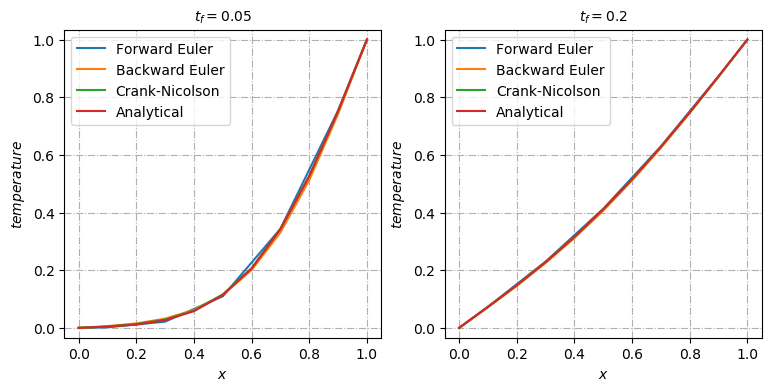
\includegraphics[scale=.6]{../Results/Comparison_1.png} 
        \caption{TR}
        \label{fig:TR}   
\end{figure}  



\begin{table}
    \centering
    \caption{\textbf{FIKS} maxerror}
\pgfplotstabletypeset[
column type=l,
every head row/.style={
before row={
\toprule &  \multicolumn{2}{c}{$\Delta x =0.1$} & \multicolumn{2}{c}{$\Delta x =0.01$}\\
},
after row=\midrule,
},
every last row/.style={
after row=\bottomrule},
columns/Method/.style ={column name=Method},
columns/t1/.style ={column name= { $  t_{f}=0.05$}},
columns/t2/.style={column name={ $  t_{f}=0.2$}},
columns/t3/.style={column name={ $  t_{f}=0.05$}},
columns/t4/.style={column name={ $  t_{f}=0.2$}},
col sep=&,row sep=\\,
string type,
]{
Method & t1 & t2 & t3 & t4 \\  
fw&$5 \cdot 10^{-1}$ & $2.2 \cdot 10^{-2}$ & $5.1 \cdot 10^{-3}$ & $4.3 \cdot 10^{-4}$\\ 
bw&$5.5 \cdot 10^{-1}$ & $2 \cdot 10^{-2}$ & $7.9 \cdot 10^{-3}$ & $2 \cdot 10^{-5}$\\ 
cn&$2 \cdot 10^{-1}$ & $2.6 \cdot 10^{-3}$ & $2.5 \cdot 10^{-3}$ & $1.6 \cdot 10^{-4}$\\  }
\end{table}

\begin{table}
    \centering
    \caption{\textbf{FIKS} average}
\pgfplotstabletypeset[
column type=l,
every head row/.style={
before row={
\toprule &  \multicolumn{2}{c}{$\Delta x =0.1$} & \multicolumn{2}{c}{$\Delta x =0.01$}\\
},
after row=\midrule,
},
every last row/.style={
after row=\bottomrule},
columns/Method/.style ={column name=Method},
columns/t1/.style ={column name= { $  t_{f}=0.05$}},
columns/t2/.style={column name={ $  t_{f}=0.2$}},
columns/t3/.style={column name={ $  t_{f}=0.05$}},
columns/t4/.style={column name={ $  t_{f}=0.2$}},
col sep=&,row sep=\\,
string type,
]{
Method & t1 & t2 & t3 & t4  \\  
fw&$9.6 \cdot 10^{-2}$ & $6.5 \cdot 10^{-3}$ & $9.9 \cdot 10^{-4}$ & $1.8 \cdot 10^{-4}$\\ 
bw&$1.2 \cdot 10^{-1}$ & $9.4 \cdot 10^{-3}$ & $1.9 \cdot 10^{-3}$ & $1.3 \cdot 10^{-5}$\\ 
cn&$4.5 \cdot 10^{-2}$ & $1.3 \cdot 10^{-3}$ & $6.5 \cdot 10^{-4}$ & $8.5 \cdot 10^{-5}$\\  }
\end{table}

\bibliography{ref}
\bibliographystyle{plain}


\end{document}





% ------------------- end of main content ---------------



